\documentclass[11pt,a4paper]{article}

\usepackage[T1]{fontenc}
\usepackage[utf8]{inputenc}
\usepackage{lmodern}
\usepackage[margin=2.4cm]{geometry}
\usepackage{amsmath,amssymb,amsthm,bm,mathtools}
\usepackage{booktabs,array,tabularx,multirow}
\usepackage{graphicx}
\usepackage{enumitem}
\usepackage{xcolor}
\usepackage{tikz}
\usetikzlibrary{arrows.meta,decorations.pathreplacing,calc,patterns,positioning}
\usepackage{xr-hyper}
\usepackage[colorlinks=true,linkcolor=teal!70!black,citecolor=teal!70!black,urlcolor=teal!70!black]{hyperref}
\usepackage{caption}
\captionsetup{font=small,labelfont=bf}
% Labels of the supplementary file are referenced with the prefix S-.
\externaldocument[S-]{paper1_supplement}[paper1_supplement.pdf]

\theoremstyle{plain}
\newtheorem{theorem}{Theorem}
\newtheorem{proposition}{Proposition}
\newtheorem{lemma}{Lemma}
\newtheorem{corollary}{Corollary}
\theoremstyle{definition}
\newtheorem{definition}{Definition}
\newtheorem{counterexample}{Counterexample}
\theoremstyle{remark}
\newtheorem{remark}{Remark}

\setlength{\parskip}{0.4em}
\setlength{\parindent}{0pt}
\newcommand{\nj}{\textsc{nj}}
\newcommand{\nh}{\textsc{nh}}
\newcommand{\tcross}{\tau_{\mathrm{cross}}}
\newcommand{\pred}{\operatorname{pred}}
\newcommand{\R}{\mathbb{R}}
\newcommand{\Pb}{\mathcal{P}}
\newcommand{\Psim}{\Pb^{\mathrm{sim}}}
\newcommand{\Pd}{\Pb_\Delta}
\newcommand{\Fpi}{\overline F_\Pi}
\newcommand{\I}{\mathcal I}
\newcommand{\Supp}[1]{Supplementary Section~\ref{S-#1}}

\title{\textbf{Scheduling a Shared Mobile Head Across Parallel Conveyors with Endogenous Blocking}\\[0.3em]
\large Formulation, properties, and a learned dispatching policy trained by expert iteration with scenario search}
\author{laser-conveyor-optimization\\\small\url{https://github.com/juanlopez-gif/laser-conveyor-optimization}}
\date{November 2026 --- short version of draft 1.3 (version 0.7.42)}

\begin{document}
\maketitle

\begin{abstract}
A shared laser head serves parts arriving on parallel conveyors. Processing a part stops
only its own conveyor, and an unprocessed part reaching the end of the working zone stops
its conveyor until served, so the schedule sets every part's availability; arrival
instants are unknown. We formulate the problem exactly in continuous time, each belt an
odometer and each part one entry coordinate; prove strong NP-hardness of its offline
maximum-lateness and total-completion-time variants with the number of conveyors in the
input, and sufficient light-traffic conditions under which every non-idling ready-only
rule is within one interception time of the offline optimum in makespan and mean flow
time; design a sampled-future look-ahead; and amortize it into a permutation-equivariant
Transformer policy trained by expert iteration. On 30 reserved realizations (seeds
7000--7029) of eight regimes, used once, the policy beat the nearest-part rule with its
legacy arrival-time tie-break by 2--7\,\% in seven regimes of each dispatch mode
(individual 95\,\% intervals; Holm: six in B, seven in C). In a retrospective rerun with the observable tie-break on the
same realizations, it beat the rule in every tested regime (2.0--7.6\,\%, the margin close
to zero at heavy load, Poisson arrivals, slow head). No difference from its expert was
detected (no equivalence margin set). It decides in 10.8~ms (median, one thread, fully
loaded machine; above the design's 5~ms budget in about 98\,\% of the decisions on that
machine) against 1.2~s for the search. The distance to the optimum is not measured.
\end{abstract}

%====================================================================
\section{Introduction}
%====================================================================
Cells in which one shared actuator serves several moving streams are common in sorting,
packaging and marking lines \cite{S01_Mattone2000,S02_Han2020,S03_Nielsen2023,S04_Schettini2023}.
In most of them the belt never stops for the actuator: an item that is not picked in time
leaves the window and is lost, and the scheduling problem is an interception problem with
fixed availability windows. Conveyor stops caused by unfinished work are classical in
mixed-model assembly lines, where a stop shifts every later product
\cite{Xiaobo2000,Tamura2011}; there, however, each station has its own worker, the launch
sequence is fixed offline, and a stop halts the whole line. The cell studied here is
different in a way that changes the problem's structure. A laser head marks parts on three
parallel conveyors; marking a part stops its conveyor for the processing time, and a part
that reaches the end of the laser zone unmarked stops its conveyor until the head serves
it. Every decision therefore moves the availability windows of the other parts on the same
belt, and a late decision creates blocking that propagates. Parts keep arriving while the
cell runs, at rates the controller knows but at instants it does not, and the controller
observes only the parts on the belts.

We state the problem, establish what is known about it, and solve its online version with
a learned policy whose quality we measure on reserved realizations. The contributions are:
\begin{enumerate}[nosep]
\item An exact continuous-time formulation (Section~\ref{sec:problem}) in which each
  conveyor is a belt odometer and each part one entry coordinate, so that positions,
  interception, processing stops and blocking are all implicit in the start times; the
  online problem with its information model, including an observable tie-break rule
  (Section~\ref{sec:online}); and a time-indexed MILP (\Supp{app:milp}).
\item The properties of the problem (Section~\ref{sec:properties}): strong NP-hardness of
  the offline maximum-lateness and total-completion-time variants with the number of
  conveyors in the input; belt order natural but not dominant; valid lower bounds that
  account for the belt kinematics, with their measured quality; and sufficient conditions
  for a light-traffic regime in which every non-idling ready-only rule produces the same
  schedule, within one interception time of the offline optimum in makespan and mean flow
  time.
\item A look-ahead search (Section~\ref{sec:search}) that simulates every candidate against
  sampled futures of the unknown arrivals and scores it by the realized unpenalized flow
  time of all parts.
\item A learned dispatching policy (Section~\ref{sec:policy}) that reads the state as a set
  of tokens, points to any candidate part, and is trained by expert iteration with the
  scenario search as expert on cells with one to six conveyors; and its confirmatory
  evaluation on reserved realizations under a protocol frozen before the run
  (Section~\ref{sec:confirm}).
\end{enumerate}
A companion paper (Paper~2) uses the policy and the nearest-part rule as controllers to
measure the value of upstream visibility and of pre-positioning; this paper is about the
problem and the decision method. Proofs, the MILP, the design study of the search, all
development results and further evaluation material are in the supplementary file.

%====================================================================
\section{Related work}\label{sec:related}
%====================================================================
\textbf{Picking and sorting from moving conveyors.} With one arm over one belt and Poisson
arrivals, \cite{S02_Han2020} sequence the reachable objects by dynamic programming and show
that first-in and nearest-first are not optimal in general; sorting on a moving belt
\cite{S01_Mattone2000} and value-aware sorting with availability windows
\cite{S05_Kokkalis2026} share that setting. With several arms, \cite{S03_Nielsen2023} batch
items from an infeed into tray lanes inside a 1.8~s decision budget, and
\cite{S04_Schettini2023} schedule identical robots along input and output conveyors by row
generation and local search. A robot that always takes the foremost item of one of several
accumulating infeeds, with no release times and no belt stops, is polynomial for a fixed
number of infeeds \cite{Li2026}. In all of these the windows are exogenous; where conveyor
motion is a decision, as for the output conveyor of \cite{S04_Schettini2023}, it is a
separate control lever rather than a consequence of the processing.

\textbf{Interception and blocking.} The moving-target travelling salesman problem
\cite{S06_Helvig2003}, its formulations with visibility windows \cite{S07_Stieber2022} and
over a graph of convex sets \cite{S08_Philip2024} model a single agent intercepting targets
with exogenous velocities, offline; our formulation uses the same geometry with endogenous
motion. Blocking as a schedule-dependent loss appears in packaging machines
\cite{S10_Briskorn2025} and in a warehouse whose full crane buffers stop the upstream
conveyors \cite{S11_SalviaHornos2026}, both minimised offline; single-machine scheduling
with release dates, from which our complexity result is inherited, is classical
\cite{Lenstra1977,Schrage1968,Baker1974}.

\textbf{Mixed-model assembly lines.} Work that cannot be finished inside a station is
either left to utility workers while the line keeps moving \cite{Yano1991,Tsai1995,Sarker2001},
or stops the conveyor until it is done \cite{Xiaobo2000,Tamura2011}. In the first case the
windows are exogenous; in the second a stop halts every station at once and shifts every
later product, and sequencing is strongly NP-hard already for one station
\cite{Tsai1995,Xiaobo2000}. In all of them each station has its own worker and the decision
is the launch order, fixed offline.

\textbf{Rollout and learned dispatching.} Our look-ahead is a rollout
\cite{M02_Bertsekas1997}. In conveyor cells a rollout with truncated simulated futures has
chosen the acceleration of the output conveyor of a picking line \cite{Righettini2025}, and
sampled completions of the unseen infeed queues, combined by a vote on the first action,
bring an item-sorting robot close to its full-information optimum \cite{Li2026}. Learned
dispatching includes policy-gradient methods with objective-aligned rewards
\cite{S19_Zhang2020,S21_Sun2023}, offline learning from constraint-programming schedules
\cite{S20_VanRemmerden2025}, look-ahead-based learning for robotic flow shops
\cite{S14_Kim2023}, action masking \cite{M04_Huang2022,S18_Wei2024}, and learned control of
conveyor-fed robotic cells \cite{S15_Zisgen2025,S16_Drijver2023,S17_Drakaki2017,S12_Wang2004,S13_Li2020}.
Our training loop is expert iteration \cite{Anthony2017,Silver2018} with the
state-distribution correction of \cite{Ross2011}; a policy-gradient baseline
\cite{Schulman2017} on the same representation is reported in \Supp{sec:ppo}.

\textbf{What is new.} One mobile head serves several parallel belts, every service stops
only the belt it serves, so the relative positions of the belts change with each decision
(Section~\ref{sec:problem} gives a two-belt example), and the decision is taken online
among the parts in view. The variant in which every service stops all conveyors
($\sigma\equiv1$) recovers a line-wide stop. \Supp{sec:relatedfull} gives the finer
comparisons.

%====================================================================
\section{The problem}\label{sec:problem}
%====================================================================
\subsection{System and notation}
Figure~\ref{fig:cell} shows the cell. $K=\{1,\dots,N\}$ are the conveyors; $J$ the parts of
an instance, $n=|J|$; $J_k\subseteq J$ the parts of conveyor $k$, indexed in arrival order,
$m_j\in\{0,1,\dots\}$ the index of part $j$ on its conveyor $k(j)$, and $\pred(j)$ the part
of $J_{k(j)}$ that arrived immediately before $j$. Table~\ref{tab:params} gives the
parameters and their values in the reference cell.

\begin{figure}[t]
\centering
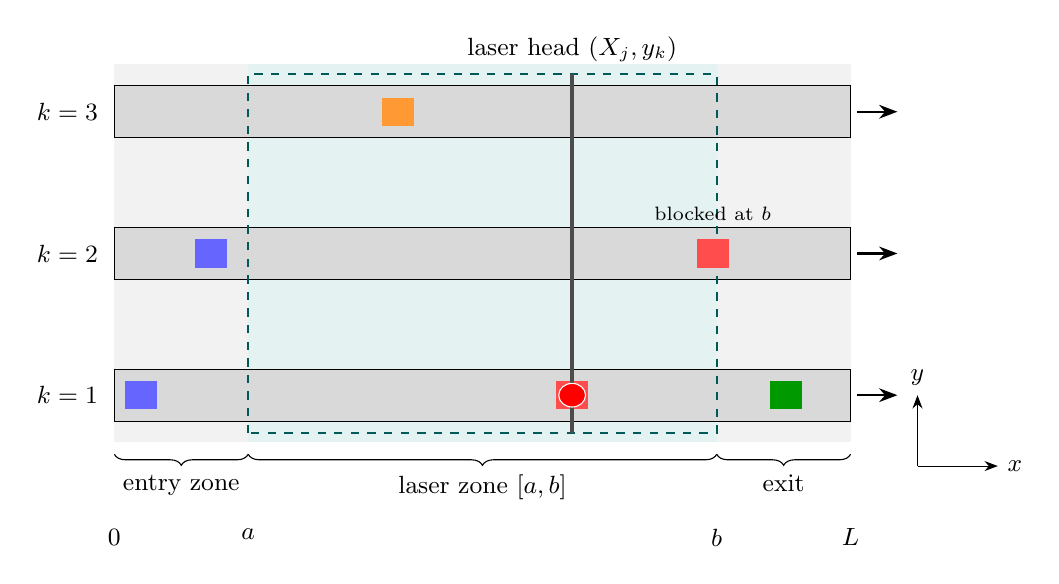
\begin{tikzpicture}[x=0.17cm,y=0.15cm,>=Stealth]
  \fill[gray!10] (0,-4) rectangle (10,28);
  \fill[teal!10] (10,-4) rectangle (45,28);
  \fill[gray!10] (45,-4) rectangle (55,28);
  \foreach \y/\n in {0/1,12/2,24/3}{
    \draw[fill=gray!30] (0,\y-2.2) rectangle (55,\y+2.2);
    \node[left] at (-0.5,\y) {\small $k=\n$};
    \draw[->,thick] (55.5,\y) -- (58.5,\y);
  }
  \draw[teal!70!black,dashed,thick] (10,-3.2) rectangle (45,27.2);
  \fill[blue!60] (0.8,-1.2) rectangle (3.2,1.2);
  \fill[blue!60] (6,10.8) rectangle (8.4,13.2);
  \fill[orange!80] (20,22.8) rectangle (22.4,25.2);
  \fill[red!70] (33,-1.2) rectangle (35.4,1.2);
  \fill[red!70] (43.5,10.8) rectangle (45.9,13.2);
  \fill[green!60!black] (49,-1.2) rectangle (51.4,1.2);
  \draw[very thick,gray!60!black] (34.2,-3.2) -- (34.2,27.2);
  \draw[fill=red,draw=white] (34.2,0) circle (1.0);
  \node[above] at (34.2,27.4) {\small laser head $(X_j,y_{k})$};
  \node[above,font=\scriptsize] at (44.7,14) {blocked at $b$};
  \draw[decorate,decoration={brace,mirror,amplitude=4pt}] (0,-5) -- (10,-5)
       node[midway,below=4pt] {\small entry zone};
  \draw[decorate,decoration={brace,mirror,amplitude=4pt}] (10,-5) -- (45,-5)
       node[midway,below=4pt] {\small laser zone $[a,b]$};
  \draw[decorate,decoration={brace,mirror,amplitude=4pt}] (45,-5) -- (55,-5)
       node[midway,below=4pt] {\small exit};
  \node[below] at (0,-10.5) {\small $0$};
  \node[below] at (10,-10.5) {\small $a$};
  \node[below] at (45,-10.5) {\small $b$};
  \node[below] at (55,-10.5) {\small $L$};
  \draw[->] (60,-6) -- (66,-6) node[right] {\small $x$};
  \draw[->] (60,-6) -- (60,0) node[above] {\small $y$};
\end{tikzpicture}
\caption{The reference cell (top view). Parts travel in $+x$; the head reaches
$W=[a,b]\times[\min_k y_k,\max_k y_k]$ and is processing the part on belt~1 (red), whose
belt is stopped; the part on belt~2 has reached $b$ unprocessed and blocks its belt. The
controller sees the parts on the belts (entry zone, seen but not reachable, and laser zone)
but not the queue upstream of the feed point.}
\label{fig:cell}
\end{figure}

\begin{table}[t]
\centering\small
\caption{Parameters of the model and their values in the reference cell.}
\label{tab:params}
\begin{tabularx}{\linewidth}{@{}l X r@{}}
\toprule
symbol & meaning & reference cell\\
\midrule
$r_j$ & arrival (release) time of part $j$ at the feed point & arrival process\\
$p_j$ & processing time & $2.5$ s\\
$y_k$ & transverse position of conveyor $k$ & $0,12,24$ cm\\
$v_k$ & conveyor speed & $3$ cm/s\\
$a,\ b$ & start and end of the laser zone along the belt & $10,\ 45$ cm\\
$L$ & belt length (exit point) & $55$ cm\\
$\delta$ & minimum spacing between consecutive parts on a belt & $4$ cm\\
$v_x,\ v_y$ & head axis speeds & $10,\ 10$ cm/s\\
$P_0=(x_0,y_0)$ & initial head position & workspace centre\\
$\sigma_{kk'}\in\{0,1\}$ & $1$ if processing a part of conveyor $k'$ stops conveyor $k$ & $\sigma=I$\\
$\lambda_N,\ \lambda_T$ & blocking penalty per event and per blocked conveyor-second & $10$ s, $1$ s\\
$\lambda_k$ & arrival rate of conveyor $k$ (online model) & $\tfrac1{10},\tfrac1{12},\tfrac1{14}$ s$^{-1}$\\
$G$ & distribution of the processing time (online model) & constant $2.5$ s\\
$T_A$ & arrival horizon of an episode & $300$ s\\
\bottomrule
\end{tabularx}
\end{table}

We assume $\sigma_{kk}=1$ for all $k$: a part never moves while it is processed. The rule
$\sigma=I$ stops only the conveyor carrying the part; $\sigma\equiv1$ stops all conveyors.
For $P=(x,y)$ and $Q=(x',y')$, with $\Delta x=|x'-x|$ and $\Delta y=|y'-y|$, the head's
travel time is
\begin{equation}\label{eq:tau}
\tau(P,Q)=
\begin{cases}
\max\!\left(\dfrac{\Delta x}{v_x},\dfrac{\Delta y}{v_y}\right) & \text{simultaneous axes (reference cell)},\\[1.5ex]
\dfrac{\Delta x}{v_x}+\dfrac{\Delta y}{v_y} & \text{sequential axes;}
\end{cases}
\end{equation}
both are metrics, so $\tau$ satisfies the triangle inequality (the path length used by the
MILP is in \Supp{sec:formdetails}).

\subsection{Belt odometer and entry coordinates}
\begin{definition}[Belt odometer]
For each conveyor $k$ let $u_k(t)\in\{0,1\}$ be its run indicator. The odometer
$D_k(t)=v_k\int_0^t u_k(s)\,ds$ is the total distance travelled by belt $k$ up to time
$t$; it is continuous and non-decreasing.
\end{definition}
All parts on a belt move rigidly with it, so a part is fully described by one constant,
its \emph{entry coordinate} $E_j$, the odometer reading when it is placed at $x=0$. A part
can enter only once the previous one has moved at least $\delta$ away from the entry:
\begin{equation}\label{eq:entry}
E_j=\max\bigl(D_{k(j)}(r_j),\ E_{\pred(j)}+\delta\bigr),\qquad E_{\pred(j)}:=-\infty\ \text{for the first part,}
\end{equation}
\begin{equation}\label{eq:pos}
x_j(t)=\max\bigl(0,\ D_{k(j)}(t)-E_j\bigr),\qquad t\ge r_j .
\end{equation}
The maximum in \eqref{eq:entry} models the upstream queue. The entry time is
$e_j=\min\{t\ge r_j:\ D_{k(j)}(t)\ge E_j\}$ and the time the part enters the laser zone is
$R_j=\min\{t:\ x_j(t)\ge a\}$. Iterating \eqref{eq:entry} gives, for $h\preceq_k j$ (both on
$k$, $m_h\le m_j$),
\begin{equation}\label{eq:iter}
E_j\ \ge\ E_h+(m_j-m_h)\,\delta\ \ge\ D_k(r_h)+(m_j-m_h)\,\delta .
\end{equation}

\subsection{Decisions and constraints}
The decisions are a permutation $\pi$ of $J$ (the processing order of the head), the start
times $S_j\ge0$ with $C_j=S_j+p_j$, and the run/stop controls $u_k(\cdot)$, which (C5)
determines from the others. The processing position and point of part $j$ are
\begin{equation}\label{eq:X}
X_j=D_{k(j)}(S_j)-E_j,\qquad P_j=(X_j,\ y_{k(j)}).
\end{equation}
\begin{description}[nosep]
\item[(C1) Reachability.] $a\le X_j\le b$ for all $j$.
\item[(C2) One part at a time, with interception.]
  \begin{equation}\label{eq:C2}
  S_{\pi(1)}\ge\tau\bigl(P_0,P_{\pi(1)}\bigr),\qquad
  S_{\pi(i+1)}\ge C_{\pi(i)}+\tau\bigl(P_{\pi(i)},P_{\pi(i+1)}\bigr),\quad i=1,\dots,n-1.
  \end{equation}
  Since $P_{\pi(i+1)}$ depends on $S_{\pi(i+1)}$ through $D_k$, the inequality is implicit:
  the head reaches the point where the \emph{moving} part will be at $S_{\pi(i+1)}$ no later
  than the part. By the triangle inequality processing intervals are disjoint.
\item[(C3) Conveyors stop during processing.] $u_k(t)=0$ for $t\in[S_j,C_j)$ whenever
  $\sigma_{k\,k(j)}=1$.
\item[(C4) Blocking.] An unprocessed part is never carried beyond $b$:
  $D_{k(j)}(t)-E_j\le b$ for all $t\le S_j$, equivalent to $X_j\le b$: a conveyor
  \emph{must} stop when its most downstream unprocessed part reaches $b$.
\item[(C5) Non-idling conveyors.] A conveyor stops only when (C3) or (C4) forces it:
  \begin{equation}\label{eq:C5}
  u_k(t)=0\ \Longrightarrow\
  \bigl(\exists j:\ \sigma_{k\,k(j)}=1,\ t\in[S_j,C_j)\bigr)\ \lor\
  \bigl(\exists j\in J_k:\ S_j>t,\ D_k(t)-E_j=b\bigr).
  \end{equation}
  Dropping (C5) gives the relaxed model $\Pb^R$.
\item[(C6) Workspace.] $P_j\in W$ follows from (C1), and straight moves between points of
  the convex set $W$ stay in $W$.
\end{description}

\subsection{Objective}
The formulation supports the makespan, the total flow and waiting times, the maximum
lateness $L_{\max}=\max_j(C_j-d_j)$, the travel distance, the conveyor downtime and the
throughput (\Supp{sec:formdetails}). A blocked conveyor has costs in the cell beyond the delays
it causes (restart, accumulation upstream, risk for the upstream process), so it is
penalized explicitly. Let $B_j=\min\{t:\ D_{k(j)}(t)-E_j\ge b\}$ be the time part $j$ would
reach the zone end. Part $j$ blocks its conveyor iff it gets there before the head starts
on it:
\begin{equation}\label{eq:block}
\beta_j=\mathbb 1[S_j>B_j],\qquad N_B=\sum_j\beta_j,\qquad T_B=\sum_j(S_j-B_j)^+ ,
\end{equation}
and the blocking penalty is $\Pi=\lambda_N N_B+\lambda_T T_B$. The objective of this paper
is the \emph{penalized flow time}
\begin{equation}\label{eq:J}
\Fpi=\frac1n\Bigl(\sum_j(C_j-r_j)+\Pi\Bigr),
\end{equation}
the total cost per part in seconds. The weights are placeholders in equivalent seconds
until the cost of a stopped conveyor is known; the sensitivity of the conclusions to them is
not measured in this paper.

\subsection{Pre-positioning, restricted model and problem statement}
Constraint (C2) allows the head to move towards a part \emph{before} it reaches the laser
zone. A cell whose controller dispatches the head only to parts already inside the zone
satisfies in addition
\begin{equation}\label{eq:C7}
\textbf{(C7)}\qquad S_{\pi(i+1)}\ \ge\ \max\bigl(C_{\pi(i)},\,R_{\pi(i+1)}\bigr)+\tau\bigl(P_{\pi(i)},P_{\pi(i+1)}\bigr),
\qquad S_{\pi(1)}\ge R_{\pi(1)}+\tau(P_0,P_{\pi(1)}).
\end{equation}
The problems are
\begin{equation}\label{eq:P}
(\Pb)\qquad \min_{\pi,\,S,\,u}\ \Fpi(\pi,S,u)\quad\text{s.t.}\quad
\eqref{eq:entry},\ \eqref{eq:X},\ \text{(C1)--(C5)};\qquad
(\Psim)=(\Pb)+\text{(C7)}.
\end{equation}
$\Pb$ is a relaxation of $\Psim$, so its optimum bounds the cost of every non-anticipating
controller (a single part arriving at $t=0$ completes at $5.83$~s in $\Pb$ and at $7.19$~s
in $\Psim$). The cell has two action modes: \texttt{none} (basic mode B), whose candidates
are the ready unassigned parts $\mathcal R(t)$ inside the zone, and \texttt{when\_idle}
(design mode C), whose candidates are $\mathcal R(t)$ if non-empty and otherwise the
unassigned parts in the entry zone of a running belt, so that the idle head may
pre-position; it requires the camera to see the entry zone. A \emph{dispatch event} is an
instant at which the head is free and the candidate set is non-empty. Once $\pi$ is fixed,
a deterministic forward pass $\Phi:\pi\mapsto(S,u)$, which is what the simulator computes,
gives the earliest schedule compatible with (C1)--(C5) and (C7). \Supp{sec:formdetails}
gives the commitment rules, and \Supp{app:milp} a time-indexed MILP of $\Pb$, a
formulation exact up to the step for the flow-time and makespan objectives and an
unvalidated approximation for the blocking penalty; the project's CP-SAT model implements
its grid version for the makespan, the mean flow time and the mean waiting time.

\subsection{A decision moves a part on another belt}\label{sec:example}
Reference cell, two belts at $y=0$ and $12$~cm. At $t=0$ the head is free at $(38,6)$;
parts $A$ and $C$ are on belt~1 at $x=40$ and $12$~cm, part $B$ on belt~2 at $x=30$~cm.
Serving $A$ first, the head meets it at $0.6$~s and belt~1 stops; at $t=3$~s, $C$ is at
$13.8$~cm. Serving $B$ first, belt~1 keeps moving until $A$ reaches $b$ at $5/3$~s and
blocks it; at $t=3$~s, $C$ is at $17.0$~cm. The arrivals are the same and both first
services are still in progress: a choice between two parts changes the position of a third
one by 3.2~cm. The choice can also move the opening of a window: with $C$ at $x=6$~cm
instead, upstream of $a$, serving $B$ first lets $C$ reach $a$ at $4/3=1.33$~s, before $A$
blocks belt~1 at $5/3$~s, while serving $A$ first stops belt~1 from 0.6 to 3.1~s and $C$
reaches $a$ at 3.83~s, 2.5~s later. In the mixed-model lines of
Section~\ref{sec:related} transport timing shifts only through a common line stop, which
shifts every product at once; here a service stops only its own belt.

%====================================================================
\section{The online problem}\label{sec:online}
%====================================================================
\textbf{Policies and decision epochs.} In the cell, $r_j$ is revealed only when the part
arrives. A \emph{policy} maps the information available at a decision epoch to the next
part. The online problem is a semi-Markov decision process: decision epochs are the
dispatch events with at least two candidates (a single candidate is taken without a
decision), the action is any candidate part, and the cost accrued between epochs $t$ and
$t'$ is
\begin{equation}\label{eq:smdp}
c(t,t')=\int_t^{t'}\bigl|\{j:\ r_j\le s<C_j\}\bigr|\,ds+\lambda_T\,T_B(t,t')+\lambda_N\,N_B(t,t') ,
\end{equation}
the work in progress integrated over the interval plus the blocking charged in it. Since
$\int_0^\infty|\{j:r_j\le s<C_j\}|\,ds=\sum_j(C_j-r_j)$, the undiscounted return of an
episode is $-n\,\Fpi$, minus its total cost (the accounting of the forced initial segment,
of the draining after the last decision and of episodes without arrivals is in
\Supp{sec:formdetails}). The state of the process includes the hidden queue upstream of the
feed point and, under bursty arrivals, the phase of the source; a policy acts on the
observation $\I_t$ below, which omits both, so $\I_t$ need not be a Markov state.

\subsection{Information model and the observable tie-break}\label{sec:info}
A policy may use only what the cell observes. Let $O(t)\subseteq J$ be the parts observable
at $t$ and $o_j$ the instant from which part $j$ is observable. The information at a
decision epoch is
\begin{equation}\label{eq:info}
\I_t=\Bigl(t,\ \text{head state},\ \text{belt states},\
\bigl\{(k(j),x_j(t),o_j,p_j,\text{status}_j):\ j\in O(t)\bigr\},\ \theta,\ T_A\Bigr),
\end{equation}
where $\theta$ are the cell's parameters (Section~\ref{sec:general}) and $T_A$ the known
arrival horizon: the controller knows the rates $\lambda_k$ and $T_A$ but not the instants
of the future arrivals. In the reference information model (an overhead camera over the
belts) $O(t)$ is the set of parts on a belt, in the laser or entry zone, and $o_j=e_j$; the
arrival time $r_j$ itself is not observed, and a part that waited in the hidden queue shows
no trace of it. A look-ahead may simulate only the parts of $O(t)$ plus synthetic arrivals
drawn from $\theta$, never the real future; a test verifies that changing the real future
changes no search cost.

\textbf{Tie-break.} Rules that rank candidates by travel time compare the times rounded to
$10^{-9}$~s and break exact ties by $o_j$, then by part number. Exact ties are frequent
(equal lane moves, several parts stopped at $b$), so the tie rule is part of the
definition of a policy, and it must use observable quantities only. Up to and including the
confirmatory run of Section~\ref{sec:confirm}, the rules and the candidate ranking of the
known-parts search broke ties by the real arrival time $r_j$ instead (the \emph{legacy
key}), which is not observed (an external review found it); the network's own decisions
never used it. On 30 development realizations the observable key changes 0.2--2.5\,\% of
the decisions of the rules and 0.1--1.3\,\% of those of the search, and moves their paired
cost by at most $\pm1.5$\,\% per regime, of either sign (\Supp{sec:formdetails}). The
prespecified confirmatory numbers are kept as they were; the comparators were rerun
afterwards on the same reserved realizations with both keys, as a retrospective
sensitivity analysis (Section~\ref{sec:confirm}).

\subsection{The general stochastic problem}\label{sec:general}
The learned policy targets a family of cells. A cell is the parameter vector
\begin{multline*}
\theta=\bigl(N,\ (y_k,v_k,\lambda_k)_{k=1}^N,\ G,\ v_x,v_y,\ \text{motion model},\\
a,b,L,\delta,\ \sigma,\ \lambda_N,\lambda_T,\ \text{pre-positioning mode},\ \text{observation level}\bigr).
\end{multline*}
Given $\theta$, the arrivals of conveyor $k$ form a Poisson process of rate $\lambda_k$ or
an on/off Poisson source with the same mean rate, independent between conveyors; processing
times are i.i.d.\ with distribution $G$. An instance $\omega$ is a realization up to $T_A$,
after which the system drains. Policies are selected and compared by the mean paired ratio
to the nearest-part rule \nj\ on the same realizations (common random numbers),
\begin{equation}\label{eq:general}
\min_\mu\ \mathbb E_{\theta\sim\Theta}\,\mathbb E_\omega\Bigl[\frac{\Fpi(\mu;\theta,\omega)}{\Fpi(\mu_{\nj};\theta,\omega)}\Bigr],
\end{equation}
estimated by the mean over realizations of the paired per-episode ratio, with a normal
95\,\% interval. The reference cell has processing load $\rho_p=\sum_k\lambda_k\mathbb E[p]=0.64$
and effective head load $\rho\approx0.9$ (travel included); its heavy variant has
$\rho_p=0.93$ and is overloaded.

%====================================================================
\section{Properties}\label{sec:properties}
%====================================================================
The proofs are in \Supp{app:complexity}--\Supp{app:special}; the statements use only
that $D_k$ is non-decreasing with slope at most $v_k$, \eqref{eq:entry} and (C1)--(C4), so
every bound holds for every feasible schedule of $\Pb$, hence of $\Pb^R$, of $\Psim$, of
every policy and of the decoder $\Phi$.

\begin{proposition}[Rigid belts]\label{prop:rigid}
On each conveyor the order of the parts never changes and, once two parts $i$ (earlier)
and $j$ have entered, $x_i(t)-x_j(t)=E_j-E_i\ge\delta$. The head may in general process them
in either order; $i$ must precede $j$ when $a+(m_j-m_i)\delta>b$ (the forced predecessors
$F_j$; nine positions in the reference cell). This condition is sufficient, not necessary:
release times and the realized belt motion can force further precedences; the bounds use
only the sufficient set and remain valid.
\end{proposition}
\begin{proposition}[Blocking cascade]\label{prop:cascade}
On conveyor $k$ at time $t$ the binding cap is set by the most downstream unstarted part:
$D_k(t)\le\min\{E_j+b:\ j\in J_k,\ S_j>t\}$. Processing the parts of a conveyor out of belt
order therefore tends to cause blocking.
\end{proposition}
\begin{proposition}[Feasibility]\label{prop:feasible}
With blocking, $\Pb$ is always feasible: even if $v_k\ge v_x$ the part stops at $b$ by (C4)
and is then reachable.
\end{proposition}
Belt order is therefore natural, but \emph{not} dominant (Section~\ref{sec:special}), so the
policy of Section~\ref{sec:policy} may point to any candidate, not only to belt heads.

\begin{proposition}[Complexity]\label{prop:complexity}
With the stop rule $\sigma=I$ and the number of conveyors $N$ part of the input, the
decision versions of the offline problem $\Pb$ for $L_{\max}$ and for $\sum_jC_j$
(equivalently $\sum_jF_j$) are NP-hard in the strong sense.
\end{proposition}
The reduction is from $1\,|\,r_j\,|\,\sum C_j$ \cite{Lenstra1977} and
$1\,|\,r_j\,|\,L_{\max}$ (strong version from 3-PARTITION, stated and proved in
\Supp{app:complexity}), with one part per conveyor. Not covered: a fixed number of
conveyors, the all-conveyors stop rule, the makespan and the penalized objective. In
Graham-style notation the problem is
\[
1\ \big|\ r_j,\ s_{ij}(t,z),\ \text{blocking},\ \text{endogenous windows}\ \big|\ C_{\max},\ \textstyle\sum F_j,\ L_{\max},
\]
with a travel setup that depends on the time and the belt state $z$.

\subsection{Lower bounds}\label{sec:bounds}
\Supp{app:bounds} proves bounds valid for every feasible schedule: (L1) an earliest start
of each part from the head's first move, its forced predecessors and the belt kinematics
since the arrival of every earlier part of its belt (which captures the upstream queue);
(L2) minimum gaps between two processings, by lane change or belt spacing; (L3) a
Jackson-type tail bound on the makespan with the gaps of any order; (L4) per-conveyor
bounds on the makespan and the ordered completion times; (L5) the preemptive SRPT
optimum \cite{Schrage1968,Baker1974} with releases (L1), a bound on $\sum_jC_j$; and (L6) a
sequence relaxation that recomputes the availability of each part from the parts processed
before it, solved \emph{exactly for the makespan} by dynamic programming over (processed
set, last part) for $n\le10$, and only bounded from below for $\sum_jC_j$. Table~\ref{tab:bounds}
gives their quality. Part of every flow-time gap can be the true difference between $\Pb$
and the non-anticipating schedules rather than looseness of the bounds; the share is not
quantified. The bounds do not enter the online method.

\begin{table}[t]
\centering\small
\caption{Quality of the lower bounds: mean gap $100\,(\mathrm{UB}-\mathrm{LB})/\mathrm{LB}$
over three random instances of the reference cell per size (Poisson arrivals at the
reference rates). For $n\le8$ the upper bound is the best of two values: the enumeration of
the $n!$ orders, each decoded by the fixed-sequence decoder $\Phi$ in the simulator at a
0.01~s step and simulated only if its L6 sequence bound is below the incumbent plus 0.1~s,
and the four online rules; it is the optimum over $\Phi$ up to the simulator's step error
and that pruning allowance, not a certified exact value. For $n\ge10$ it is the best of the
four online rules, a heuristic, so those gaps mix the bounds' looseness with the rules'
suboptimality. Unpenalized objectives; $\Phi$ dispatches the next part of its order as soon
as that part is eligible (waiting for it if another part is ready) and never moves the head
in anticipation, so these gaps are measured against the restricted model $\Psim$, not
against the optimum of $\Pb$. Last column: the time of one evaluation of all bounds.}
\label{tab:bounds}
\begin{tabular}{@{}cccc@{}}
\toprule
$n$ & makespan & mean flow time & bound time [s]\\
\midrule
6 & 4.0\,\% & 11.0\,\% & 0.03\\
8 & 4.8\,\% & 13.4\,\% & 0.03\\
10 & 5.4\,\% & 20.4\,\% & 0.08\\
20 & 7.1\,\% & 37.6\,\% & 0.11\\
40 & 3.6\,\% & 45.9\,\% & 0.25\\
\bottomrule
\end{tabular}
\end{table}

\subsection{When the rules are optimal, and when they are not}\label{sec:special}
Let $e^0_j=r_j+a/v_{k(j)}$ be the free-flow availability of part $j$, and
$I^\ast=\max\bigl((b-a)/(v_x+\min_kv_k),\ (\max_ky_k-\min_ky_k)/v_y\bigr)$ an upper bound
on the interception time of a part that has just entered the zone at $a$ on a moving belt
(2.69~s in the reference cell). It does not bound every ready part: a part already blocked
at $b$ with the head at $a$ on the same belt needs $(b-a)/v_x=3.5$~s; the conditions below
ensure that every part is met on entry.
\begin{theorem}[Light traffic]\label{thm:light}
Assume simultaneous axes, $\sigma=I$, $a\ge\delta$, $v_k\le v_x$ and $v_kI^\ast\le b-a$ for
all $k$. If consecutive parts $h,i$ of the same conveyor satisfy
$r_i\ge r_h+a/v_k+I^\ast+p_h$ and, in $e^0$-order, $e^0_{(q+1)}\ge e^0_{(q)}+I^\ast+p_{(q)}$
and $e^0_{(1)}\ge\tau(P_0,(a,y_{(1)}))$, then at every dispatch event exactly one part is
ready (there is no decision epoch), every non-idling policy that dispatches among the parts
ready in the zone with the earliest interception (mode \texttt{none}; not a policy that
pre-positions the idle head) produces the same schedule, and that schedule satisfies
$e^0_j\le S_j\le e^0_j+I^\ast$; its makespan and mean flow time exceed the optimum of $\Pb$
by at most $I^\ast$. Under the weaker conditions $r_i\ge r_h+a/v_k+p_h$,
$e^0_{(q+1)}\ge e^0_{(q)}+p_{(q)}+|y_{(q+1)}-y_{(q)}|/v_y$ and
$e^0_{(1)}\ge\tau(P_0,(a,y_{(1)}))$, the schedule $S_j=e^0_j$ with the head pre-positioned at
$(a,y_{k(j)})$ is feasible for $\Pb$ and optimal for every regular objective, and the bound
of Section~\ref{sec:bounds} is exact.
\end{theorem}
The conditions are sufficient, not necessary. In the reference cell the first ones need
inter-arrivals of at least 8.5~s per conveyor and 5.2~s between consecutive availabilities,
so the reference instances are contended. Outside them the rules are not optimal in
general (\Supp{app:special}, each instance reproduced by a test):
\begin{itemize}[nosep]
\item \emph{Belt order is not optimal for the flow time}: on a single conveyor a short part
  1.5~s behind a long one should go first, gaining about 2~s per part
  (Counterexample~\ref{S-cex:single}).
\item \emph{Waiting beats serving}: waiting 0.2~s for a part on the head's own belt improves
  the makespan by 1~s and the mean flow time by 0.4~s; no implemented rule idles
  deliberately (Counterexample~\ref{S-cex:wait}).
\item \emph{Anticipation pays}: for a single part the optimum of $\Pb$ pre-positions the head
  and completes at 5.83~s, every ready-only policy at 7.19~s ($+23$\,\%)
  (Counterexample~\ref{S-cex:anticipation}).
\item \emph{Delaying a start of the same sequence} never relaxes the successor's travel
  constraint (Proposition~\ref{S-prop:delay}); whether it can pay through the belt is open.
\end{itemize}
On 30 random five-part instances of the reference cell, enumerated over all 120 orders,
first-in was optimal in 21--22 and nearest-part in 20--21: the rules are good and not
optimal, which is the room the online method works in.

%====================================================================
\section{The look-ahead search}\label{sec:search}
%====================================================================
\textbf{Rollout over the known parts.} The first search is a fortified rollout
\cite{M02_Bertsekas1997} on the cell's exact event-driven simulator. At a decision epoch
with candidate set $\mathcal C$ and base policy $\mu$, it keeps $K=6$ candidates, ranked by
interception time when $\mu$ is a rule and by $\mu$'s own scores when $\mu$ is the network,
always including $\mu$'s own choice; for each it clones the simulator with online
information only (the real future arrivals and the hidden queue removed), forces the
candidate, lets $\mu$ continue until every part known at the decision is processed, and
scores the sum of their completion times. It applies the best-scoring first decision and
re-plans at the next epoch, keeping the base choice on ties. With $\mu=\nj$ it is the
\emph{known-parts search} of the evaluation; with $\mu$ the current network it is the expert
of the first training stage.

\textbf{Scenario search: sampled futures, scored on every part.} The known parts are a few;
the decision that serves them best may leave the head far from the belt that will need it
next. The second search samples the unknown future: for each candidate it runs $M=8$
look-aheads, each with a different synthetic list of arrivals over the next $W=30$~s,
Poisson at the belts' known mean rates (the clone drains after $t+W$; the synthetic process
is not truncated at $T_A$), with common random numbers across candidates. The score of a
candidate is the mean over the $M$ futures of the \emph{realized cost of all parts} from the
decision on, i.e.\ the work-in-progress integral of \eqref{eq:smdp} \emph{without} the
blocking penalty: the expert scores unpenalized flow while every evaluation uses the
penalized objective $\Fpi$. These settings came from a design study on development
realizations (\Supp{sec:searchdesign}), in which sampled futures helped, among the variants tried, only
when the score counts every part, one or two futures were worse than none, and truncating the look-ahead
with a learned value was far worse than not truncating. The chosen expert costs about ten
times the known-parts rollout, 22~s per episode on the reference cell and 112~s on the
heavy variant on one worker: it is an expert, not a controller.

%====================================================================
\section{The learned policy}\label{sec:policy}
%====================================================================
\textbf{State as a set of tokens.} The policy reads $\I_t$ as an unordered set of tokens:
one per unfinished part on a belt or being processed (23 features: status, position,
times to $b$ and to interception, waiting time since the part became observable,
processing times, blocking flag, rank on the belt, candidate and committed flags, offsets
from the head, its belt's speed and state), one per conveyor (11), one for the head (9) and
one context token (21) that carries $\theta$ and the scalars of \eqref{eq:info}, including
the time left to $T_A$. No token holds a list position or a conveyor index
(\Supp{sec:policydetails} lists the features and scalings).

\textbf{Network and action.} One linear embedding per token type, a pre-norm Transformer
encoder without positional encoding, so that the output is permutation-equivariant in the
parts and the conveyors, and a masked mean $g$ over all tokens. The policy head gives a
logit $\mathrm{MLP}([h_i,g])$ to every part token; non-candidates and padding receive
$-\infty$, so the action is a pointer to \emph{any} candidate of the open decision, not only
a belt head. A value head predicts the normalized cost-to-go (used in training only). Size
S has 4 layers, $d=128$, 0.88~M parameters; M has 6.7~M and L 39~M. Single-state inference
on one thread takes 4.1~ms (median) for S on an unloaded machine.

\textbf{Expert iteration.} Training alternates data generation and fitting
\cite{Anthony2017,Silver2018}. In iteration 0 the known-parts rollout over \nj\ acts on
episodes drawn from the training distribution and labels every decision with at least two
candidates with the look-ahead costs of its candidates; the network is trained from
scratch on them. In iteration $k\ge1$ the expert is the search over
$\mathrm{net}_{k-1}$ (the scenario search from the second stage on), the acting policy is
$\mathrm{net}_{k-1}$ except that the expert acts with probability $\beta=0.3$
\cite{Ross2011}, and $\mathrm{net}_k$ is fine-tuned on a replay buffer of the last two
iterations. The policy loss is the cross-entropy to the softmin of the relative look-ahead
costs with temperature 1~s; the value loss is $0.25\times$ the MSE of the normalized
cost-to-go. After each iteration the network is scored on fixed validation cells by the
criterion \eqref{eq:general} and kept only if it improves; the run stops after two
rejections. This is policy iteration with the search as the improvement operator, not
policy-gradient learning from the reward (hyperparameters in \Supp{sec:policydetails}).

\textbf{Training distribution.}\label{sec:dist} Every training episode draws one cell: the
reference cell (25\,\%), its heavy variant (10\,\%), or a general cell (65\,\%) with
$N\in\{1,\dots,6\}$ conveyors and randomized belt speeds, processing load
$\rho_p\sim U[0.3,0.95]$ (overloaded cells included), processing-time distributions, head
speeds and motion model, geometry, penalty weights, stop rule, pre-positioning mode,
observation level and, with probability 0.5, bursty arrivals. All values reach the network
through its tokens except the burst parameters, which it must infer from what it sees.
Training and validation seeds are disjoint from each other and from the reserved seeds of
Section~\ref{sec:confirm}.

%====================================================================
\section{Development results}\label{sec:dev}
%====================================================================
Everything here was measured on development realizations with the legacy tie-break and used
to make design decisions; nothing is confirmatory (tables, figures and the full text are in
\Supp{sec:devfull}). With the known-parts expert, networks of 0.88, 6.7 and 39~M parameters
scored $-2.79$, $-2.88$ and $-2.44$\,\% against \nj\ on the validation groups, within each
other's intervals: no detectable improvement with size, from one run per size in which
size, data, episodes and iterations varied together. Continuing the S network with the
scenario search as expert moved the score from $-2.79$ to $-4.83$\,\% after two iterations,
a continuation in which the expert and further iterations changed together, so it is an
observation on one chain, not a matched ablation; after two further continuations that
extended the training mix (design mode, observation levels, bursts and slow heads) the
network frozen for the confirmatory run scored $-3.82$\,\% on four groups. An expert that
samples the cell's bursty arrival model did not improve on the Poisson one. A PPO baseline
\cite{Schulman2017} on the same tokens, mask, simulator and validation groups, trained under
a protocol fixed before the runs on the final training mix from its first episode
(whereas the expert-iteration chain changed its mix by stage), did not
reach the chain within its budget: from scratch, with a budget of 40\,000 episodes, it stayed 4--8\,\%
above \nj\ and 8--12\,\% above the frozen network on three seeds (22~minutes per run against
12.7~hours for the whole chain on the same workstation), and fine-tuning the frozen network
with PPO made it worse on all three seeds. The two methods differ in the learning signal,
the compute spent and the curriculum, which these runs do not separate.

%====================================================================
\section{Confirmatory evaluation}\label{sec:confirm}
%====================================================================
\textbf{Protocol.} The frozen network, the known-parts search over \nj, the scenario search
over the frozen network (``its expert''), \nj\ and the nearest-head rule \nh\ were run on 30
realizations reserved for this evaluation (seeds 7000--7029, shared with the companion
paper, which analyzes the same realizations for different questions), never seen by any
design decision and used once for this prespecified evaluation, on eight regimes: the
reference cell and its heavy variant, Poisson and bursty arrivals, nominal head and a head
twice as slow (\Supp{sec:confirmfull}, Table~\ref{S-tab:regimes}), in the basic mode (B)
and the design mode (C). Every policy runs on the same realizations, so every contrast is
paired; we report $\Delta=100\,(\frac{1}{30}\sum_\omega J_X(\omega)/J_Y(\omega)-1)$ for ``X vs
Y'' with a normal 95\,\% interval. Latencies are measured at every decision of the
network's episodes with at least two candidates, every policy timed on the same state (one
thread, the machine fully loaded by the other workers): 16\,215 decisions in B and 17\,147
in C. The protocol, the regimes and the contrasts were fixed before the run. The run used
the legacy tie-break for \nj, \nh\ and the known-parts search. After it, as a
\emph{retrospective sensitivity analysis, not a new confirmation}, these three comparators
(with the key applied both to the candidate ranking and inside every look-ahead) were rerun
on the same reserved realizations with both keys (every legacy rerun reproduces the
archived cost to $1.4\cdot10^{-13}$~s per part) and paired with the archived costs of the
network. A confirmation under the observable key would need fresh realizations.

\begin{table}[t]
\centering\small
\caption{Confirmatory evaluation, basic mode (B): paired $\Delta$ of the penalized flow
time of each policy against \nj; contrasts of the two searches against the network
(positive = the network is better; in parentheses the realizations in which the search is
cheaper); and per-decision latency (median / 95th percentile). Bold: the individual
interval excludes zero. Prespecified run: rules and known-parts search with the legacy
arrival-time tie-break. Seeds 7000--7029, shared with the companion paper.}
\label{tab:confirmB}
\resizebox{\linewidth}{!}{% generated by experiments/paper1_figures.py
\begin{tabular}{@{}lccc|cc|ccc@{}}
\toprule
 & \multicolumn{3}{c|}{paired $\Delta$ vs \textsc{nj} [\%]} & \multicolumn{2}{c|}{contrasts [\%]} & \multicolumn{3}{c}{latency p50 / p95 [ms]} \\
regime & known-parts & sampled-future & network & search vs net & teacher vs net & search & network & teacher \\
\midrule
real / Poisson / nominal head & {\boldmath$-4.16 \pm 1.98$} & {\boldmath$-7.60 \pm 2.17$} & {\boldmath$-7.22 \pm 1.95$} & {\boldmath$+3.35 \pm 1.10$} (1/30) & $-0.39 \pm 1.24$ (17/30) & 2.0 / 6.9 & 8.5 / 13.7 & 0.43 / 1.43 s \\
real / Poisson / slow head & {\boldmath$-3.73 \pm 2.17$} & {\boldmath$-7.72 \pm 2.14$} & {\boldmath$-7.25 \pm 1.74$} & {\boldmath$+3.83 \pm 1.56$} (3/30) & $-0.53 \pm 1.12$ (15/30) & 3.3 / 10.5 & 10.2 / 15.3 & 0.82 / 2.22 s \\
real / bursts / nominal head & $-0.57 \pm 1.54$ & {\boldmath$-2.68 \pm 1.44$} & {\boldmath$-1.96 \pm 1.74$} & $+1.54 \pm 1.60$ (6/30) & $-0.65 \pm 1.12$ (16/30) & 4.3 / 12.6 & 9.8 / 14.7 & 0.84 / 2.31 s \\
real / bursts / slow head & {\boldmath$-4.25 \pm 1.91$} & {\boldmath$-6.72 \pm 2.12$} & {\boldmath$-6.24 \pm 2.00$} & {\boldmath$+2.22 \pm 1.42$} (7/30) & $-0.48 \pm 1.22$ (16/30) & 5.1 / 13.4 & 10.9 / 16.2 & 1.14 / 2.67 s \\
heavy / Poisson / nominal head & $+0.26 \pm 1.45$ & {\boldmath$-3.68 \pm 1.58$} & {\boldmath$-2.78 \pm 1.85$} & {\boldmath$+3.31 \pm 1.87$} (9/30) & $-0.81 \pm 1.46$ (16/30) & 5.0 / 14.9 & 11.3 / 17.5 & 1.37 / 3.33 s \\
heavy / Poisson / slow head & $+2.31 \pm 2.94$ & $-1.40 \pm 2.53$ & $-1.32 \pm 2.32$ & {\boldmath$+3.86 \pm 2.86$} (9/30) & $+0.05 \pm 2.24$ (15/30) & 5.6 / 15.9 & 11.7 / 18.0 & 1.47 / 3.54 s \\
heavy / bursts / nominal head & $-1.02 \pm 1.33$ & {\boldmath$-3.56 \pm 1.74$} & {\boldmath$-3.29 \pm 1.66$} & {\boldmath$+2.46 \pm 1.36$} (2/30) & $-0.27 \pm 0.55$ (17/30) & 7.3 / 21.3 & 12.2 / 19.6 & 1.86 / 5.12 s \\
heavy / bursts / slow head & {\boldmath$-1.89 \pm 1.87$} & {\boldmath$-4.15 \pm 1.82$} & {\boldmath$-4.15 \pm 1.74$} & {\boldmath$+2.40 \pm 1.29$} (6/30) & $+0.01 \pm 0.79$ (18/30) & 6.3 / 19.9 & 11.4 / 18.6 & 1.58 / 4.44 s \\
\bottomrule
\end{tabular}
}
\end{table}

\begin{table}[t]
\centering\small
\caption{As Table~\ref{tab:confirmB}, design mode (C): every policy, including \nj, may
pre-position the idle head. Legacy tie-break; seeds 7000--7029, shared with the companion
paper.}
\label{tab:confirmC}
\resizebox{\linewidth}{!}{% generated by experiments/paper1_figures.py
\begin{tabular}{@{}lccc|cc|ccc@{}}
\toprule
 & \multicolumn{3}{c|}{paired $\Delta$ vs \textsc{nj} [\%]} & \multicolumn{2}{c|}{contrasts [\%]} & \multicolumn{3}{c}{latency p50 / p95 [ms; teacher in s]} \\
regime & known-parts & sampled-future & network & search vs net & teacher vs net & search & network & teacher \\
\midrule
real / Poisson / nominal head & {\boldmath$-3.61 \pm 2.18$} & {\boldmath$-6.83 \pm 2.40$} & {\boldmath$-7.08 \pm 2.18$} & {\boldmath$+3.85 \pm 1.61$} (4/30) & $+0.27 \pm 1.04$ (13/30) & 1.8 / 7.5 & 8.5 / 13.4 & 0.39 / 1.50 s \\
real / Poisson / slow head & {\boldmath$-3.06 \pm 2.68$} & {\boldmath$-7.09 \pm 2.60$} & {\boldmath$-7.02 \pm 2.70$} & {\boldmath$+4.44 \pm 2.07$} (5/30) & $+0.04 \pm 1.69$ (16/30) & 3.3 / 9.8 & 9.9 / 15.2 & 0.77 / 2.03 s \\
real / bursts / nominal head & $-0.74 \pm 1.10$ & {\boldmath$-2.33 \pm 1.10$} & {\boldmath$-2.04 \pm 1.05$} & {\boldmath$+1.37 \pm 1.09$} (7/30) & $-0.28 \pm 0.78$ (12/30) & 2.9 / 12.0 & 9.9 / 15.0 & 0.57 / 2.29 s \\
real / bursts / slow head & {\boldmath$-3.11 \pm 2.13$} & {\boldmath$-7.32 \pm 2.18$} & {\boldmath$-6.56 \pm 2.15$} & {\boldmath$+3.85 \pm 2.01$} (8/30) & $-0.77 \pm 0.99$ (18/30) & 4.3 / 13.3 & 10.5 / 16.2 & 0.97 / 2.72 s \\
heavy / Poisson / nominal head & $-0.86 \pm 1.82$ & {\boldmath$-3.91 \pm 1.73$} & {\boldmath$-4.14 \pm 1.62$} & {\boldmath$+3.49 \pm 1.53$} (7/30) & $+0.27 \pm 1.08$ (12/30) & 4.8 / 13.6 & 11.1 / 17.3 & 1.30 / 3.20 s \\
heavy / Poisson / slow head & $+0.42 \pm 1.94$ & $-0.10 \pm 2.05$ & $-1.64 \pm 2.72$ & $+2.52 \pm 2.73$ (10/30) & $+1.98 \pm 2.75$ (12/30) & 5.8 / 17.8 & 11.6 / 17.9 & 1.52 / 4.00 s \\
heavy / bursts / nominal head & {\boldmath$-2.21 \pm 1.37$} & {\boldmath$-4.78 \pm 1.50$} & {\boldmath$-4.53 \pm 1.38$} & {\boldmath$+2.47 \pm 0.95$} (3/30) & $-0.25 \pm 0.79$ (15/30) & 6.4 / 19.8 & 11.9 / 18.7 & 1.66 / 4.59 s \\
heavy / bursts / slow head & {\boldmath$-3.06 \pm 1.95$} & {\boldmath$-4.96 \pm 1.78$} & {\boldmath$-4.56 \pm 2.00$} & {\boldmath$+1.67 \pm 1.47$} (7/30) & $-0.32 \pm 1.25$ (16/30) & 6.0 / 19.4 & 11.0 / 18.2 & 1.44 / 4.12 s \\
\bottomrule
\end{tabular}
}
\end{table}

\textbf{Against the nearest-part rule.} In the prespecified run (legacy key) the network is
cheaper than \nj\ with an individual interval excluding zero in seven of the eight regimes
of each mode, by 2.0--7.3\,\% in B and 2.0--7.1\,\% in C (Tables~\ref{tab:confirmB} and
\ref{tab:confirmC}); Holm's adjustment over the eight regimes of each mode leaves six
detections in B and seven in C. The exception is the heavy load with Poisson arrivals and a
slow head ($-1.32\pm2.32$ in B, $-1.64\pm2.72$ in C), where with every belt queueing and a
head at 2.5~cm/s no tested policy improved on \nj\ by a detectable amount. With \nj\ rerun
under the observable key (retrospective, same realizations, network costs unchanged), the
network is cheaper with an individual interval excluding zero in all eight regimes of both
modes, by 2.0--7.6\,\% in B and 2.1--7.6\,\% in C; in that hard regime the contrasts become
$-2.09\pm1.99$ and $-2.68\pm2.50$, so \emph{the margin there stays close to zero}.

\textbf{Against the look-aheads and \nh.} The known-parts search has a higher point estimate of the cost than the
network in every regime (individual interval excluding zero in seven of eight regimes per
mode with the legacy key; seven in B and eight in C with the observable key): 1.5--3.9\,\% in B and 1.4--4.4\,\% in C with the legacy key, and, in the
retrospective rerun with the observable key, 1.4--4.7\,\% in B and 1.5--5.2\,\% in C, pooled
$+2.95$\,\% $[2.24,3.66]$ in B and $+3.21$\,\% $[2.38,4.04]$ in C (one mean per realization
over its eight regimes, interval over the 30 means); at the heavy load with Poisson arrivals
in B, with the legacy key, it shows no detected improvement over \nj\ itself (point
estimates $+0.3$ and $+2.3$\,\%, intervals containing zero). \nh\ costs more than the network with
an individual interval excluding zero in six regimes of each mode with the legacy key and,
under the observable key, by 1.4--8.2\,\% in B and 1.5--6.7\,\% in C, excluding zero in six
regimes in B and seven in C, pooled $+3.99$\,\% $[3.16,4.81]$ in B and $+4.35$\,\%
$[3.53,5.17]$ in C.
No difference between the network and its expert was detected in any regime or mode (no
equivalence margin was set, so this is not a test of equivalence): point estimates within
$\pm0.8$\,\%, except $+1.98\pm2.75$ in C at heavy load, Poisson arrivals and slow head, an
interval that admits a practically relevant difference; the search is cheaper in 12--18 of
the 30 realizations. Table~\ref{tab:summary} collects the comparators.

\begin{table}[t]
\centering\footnotesize
\caption{Against which comparators the network is cheaper, and under which conditions.
Paired $\Delta$ of the penalized flow time over the 30 reserved realizations (seeds
7000--7029, shared with the companion paper), eight regimes per mode (\{reference, heavy\}
load $\times$ \{Poisson, bursts\} $\times$ \{nominal, slow\} head); B ready-only, C
pre-positioning while idle. For \nj, $\Delta=100\,(J_{\mathrm{net}}/J_{\nj}-1)$, negative
favours the network; for the other comparators $\Delta=100\,(J_{\mathrm{comp}}/J_{\mathrm{net}}-1)$,
positive favours the network. Counts: regimes whose individual normal 95\,\% interval
excludes zero, and in parentheses the detections after Holm's adjustment over the eight
regimes of the mode (not computed for the observable \nj\ rerun). Prespecified rows come
from the evaluation used once; retrospective rows rerun the comparator on the same
realizations against the archived network costs; the scenario search, whose base policy is
the network, was not rerun. Intervals in the last column are
mean $\pm$ half-width or [lower, upper].}
\label{tab:summary}
\setlength{\tabcolsep}{3pt}
\begin{tabularx}{\linewidth}{@{}>{\raggedright\arraybackslash}p{2.25cm}>{\raggedright\arraybackslash}p{1.9cm}cccc>{\raggedright\arraybackslash}X@{}}
\toprule
 & & \multicolumn{2}{c}{excl.\ 0 (Holm)} & \multicolumn{2}{c}{range of $\Delta$ [\%]} & \\
\cmidrule(lr){3-4}\cmidrule(lr){5-6}
comparator, key & status & B & C & B & C & regimes without a detected difference\\
\midrule
\nj, legacy & prespecified & 7/8 (6) & 7/8 (7) & $-7.25\ldots-1.32$ & $-7.08\ldots-1.64$ & heavy/Poisson/slow in B ($-1.32\pm2.32$) and C ($-1.64\pm2.72$)\\
\nj, observable & retrospective & 8/8 & 8/8 & $-7.6\ldots-2.0$ & $-7.6\ldots-2.1$ & none (heavy/Poisson/slow $-2.09\pm1.99$ in B, $-2.68\pm2.50$ in C, just excluding 0)\\
\addlinespace
known-parts search, legacy & prespecified & 7/8 (7) & 7/8 (6) & $+1.54\ldots+3.86$ & $+1.37\ldots+4.44$ & B: reference/bursts/nominal ($+1.54\pm1.60$); C: heavy/Poisson/slow ($+2.52\pm2.73$)\\
known-parts search, observable & retrospective & 7/8 (7) & 8/8 (8) & $+1.43\ldots+4.65$ & $+1.50\ldots+5.24$ & B: reference/bursts/nominal ($+1.43$ $[-0.15,3.01]$)\\
\addlinespace
\nh, legacy & prespecified & 6/8 (6) & 6/8 (6) & $+0.18\ldots+9.03$ & $-0.16\ldots+7.49$ & heavy/Poisson/slow and heavy/bursts/slow in both modes\\
\nh, observable & retrospective & 6/8 (6) & 7/8 (6) & $+1.37\ldots+8.19$ & $+1.46\ldots+6.71$ & B: heavy/bursts/slow, heavy/Poisson/slow; C: heavy/Poisson/slow\\
\addlinespace
scenario search over the network (its expert; not rerun) & prespecified & 0/8 & 0/8 & $-0.81\ldots+0.05$ & $-0.77\ldots+1.98$ & all eight in both modes (no equivalence margin set)\\
\bottomrule
\end{tabularx}
\end{table}

\begin{table}[t]
\centering\small
\caption{Per-decision latency of every policy on the same decisions (one thread, machine
fully loaded), pooled over the eight regimes: 16\,215 decisions in B, 17\,147 in C (seeds
7000--7029, shared with the companion paper).}
\label{tab:latency}
\resizebox{0.85\linewidth}{!}{% generated by experiments/paper1_figures.py
\begin{tabular}{@{}lcccc|cccc@{}}
\toprule
 & \multicolumn{4}{c|}{treatment B [ms]} & \multicolumn{4}{c}{treatment C [ms]} \\
policy & p50 & p95 & p99 & max & p50 & p95 & p99 & max \\
\midrule
\textsc{nj} & 0.07 & 0.17 & 0.28 & 3.3 & 0.06 & 0.16 & 0.28 & 9.9 \\
\textsc{nh} & 0.01 & 0.07 & 0.14 & 4.7 & 0.01 & 0.06 & 0.13 & 1.2 \\
known-parts search & 4.78 & 15.99 & 24.42 & 54.1 & 4.40 & 15.56 & 23.08 & 83.6 \\
network & 10.83 & 17.53 & 25.46 & 105.9 & 10.65 & 17.19 & 24.43 & 88.2 \\
sampled-future search & 1178.59 & 3630.54 & 5385.06 & 12159.0 & 1073.71 & 3511.40 & 5094.76 & 12039.6 \\
\bottomrule
\end{tabular}
}
\end{table}

\textbf{Latency.} Pooled over the regimes (Table~\ref{tab:latency}), the network decides in
10.8~ms (median), 17.5~ms (95th percentile) and 106~ms at most, on one thread with the
machine fully loaded by 47 other workers; on this loaded machine it exceeded the design's
5~ms budget in 98.07\,\% of the decisions of B and 97.62\,\% of those of C. The 4.1~ms median
of Section~\ref{sec:policy}, on an unloaded machine, does not establish a per-decision
guarantee. The scenario search needs 1.2~s (median; 0.4--1.9~s by regime, 3.6~s at the 95th
percentile), about a hundred times the network; the known-parts search 4.8~ms and the rules
under 0.2~ms. The physical slack of the cell, the time until the next part reaches $b$, is
seconds. The latency distribution and the design-mode results are in
\Supp{sec:confirmfull}.

%====================================================================
\section{Discussion}\label{sec:discussion}
%====================================================================
\textbf{What the formulation buys.} The odometer formulation makes the endogenous part of
the problem explicit and cheap: a part is one number, the belt one monotone function, and
interception, stops and blocking are consequences of the start times. It is what the
simulator implements, what the MILP discretizes and what the lower bounds exploit. Its
properties set the terms of the online problem: the offline maximum-lateness and
total-completion-time variants are strongly NP-hard with the number of conveyors in the
input, so exactness is for small windows; belt order is natural but not dominant, so the
policy must be free to point at any part; and under the sufficient light-traffic conditions
every non-idling ready-only rule makes the same decisions, so the value of a better
decision rule is concentrated in the contended regimes, where the evaluation measures it.

\textbf{What the training runs show.} In one run per size, larger networks did not score
detectably better; after the switch to the scenario-search expert, in a continuation where
the expert and further iterations changed together, the score moved by about two points.
These are observations on one chain, not matched ablations. No detectable difference
separated the amortized policy from the search that labels its data, in development and on
the reserved realizations. The learned value head, which would make deeper or cheaper search
possible, is the part that failed: in these runs its error was of the order of the
randomness of the future, which no decision changes, and swamped the differences between
candidates.

\textbf{What the policy cannot do.} At heavy load with Poisson arrivals and a slow head the
network's margin over \nj\ is close to zero under either key; with every belt queueing, the
order in which the visible parts are served matters little and the hidden queue, which no
policy sees, is what would matter (Paper~2 measures it at 2.7--3.7\,\%). With bursts the gain
falls to 2\,\% on the reference cell, and an expert that knows the burst model does not raise
it: whether the source is on now is not in the state.

\textbf{Limits.}\label{sec:limits}
\begin{itemize}[nosep]
\item The distance to the optimum is not measured: the MILP is a formulation; the
  project's CP-SAT model implements its grid version for the makespan, the mean flow time
  and the mean waiting time, and the penalized objective is specified but neither
  implemented nor validated against the continuous model; and the lower bounds were compared with offline solutions on small instances
  only.
\item The confirmatory regimes are eight variants of one 3-belt cell; the general cells with
  one to six conveyors appear only in development validation.
\item The reserved realizations were used once for the prespecified evaluation, with legacy
  keys for the comparators; the observable-key results are retrospective reruns on the same
  realizations and need fresh ones to be confirmed.
\item Latencies are for one CPU thread of a loaded workstation and a 0.88~M-parameter model,
  above the 5~ms design budget there.
\item The PPO baseline is one protocol at one budget without a hyperparameter search; the
  known-parts look-ahead is a rollout with $K=6$, not an exact search.
\item Parts are points with a minimum spacing, the head has no acceleration, processing
  times are constant in the confirmatory regimes, and the penalty weights are placeholders.
\end{itemize}

%====================================================================
\section{Conclusions}
%====================================================================
For a shared head over parallel conveyors whose belts stop locally for the head, the
schedule determines the availability of every part. The resulting problem is strongly
NP-hard offline for maximum lateness and total completion time with the number of
conveyors in the input, naturally but not dominantly ordered by belt, and, under sufficient
light-traffic conditions, indifferent to the non-idling ready-only rule within one
interception time of the offline optimum in makespan and mean flow time. In the contended regimes, a look-ahead that
samples the unknown arrivals and scores the realized unpenalized flow time of every part,
amortized into a
permutation-equivariant pointer policy by expert iteration, decided better than the
nearest-part rule on the reserved realizations: in seven of eight regimes of each mode
against the rule with its legacy tie-break and, in the retrospective rerun with the
observable tie-break on the same realizations, in all eight, with the margin close to zero
at heavy load with Poisson arrivals and a slow head. It was also cheaper than the look-ahead
over the known parts in every regime (point estimates, under either key), and no difference
from its expert was detected (no equivalence margin set), at about a hundredth of the
expert's latency (10.8~ms per decision on a loaded machine, above the design's 5~ms budget
in about 98\,\% of the decisions there). How far all of this
is from the optimum remains open.

\bibliographystyle{plain}
\bibliography{../../literature/references,extra}

\end{document}
